\chapter[Planejamento]{Planejamento}
O cronograma, é um documento fundamental em qualquer projeto, seja ele pessoal ou um projeto de equipe. Ele consiste na formalização das atividades que se busca realizar desde o início do projeto até seu término. Além disso, o cronograma serve para orientar os envolvidos no projeto no que se refere ao que deverá ser feito no tempo atual.

Atualmente, o cronograma dos alunos da equipe de Requisitos, esta integrado com o da equipe de Modelagem de Processos, de modo que o contexto a ser trabalhado se encaixe da melhor forma possível com a metodologia escolhida.

Tendo isso em mente, a ferramenta escolhida para contrução do cronograma foi o Gantter que se trata de uma aplicação web vinculada ao Google Drive que possibilita alem da criação de uma ordem de execução de tarefas, a definição de responsáveis de conclusão dessas tarefas e visualizar o grau de conclusão via porcentagem.

Neste primeiro ponto do cronograma, as atividades consistiam em fundamentar conceitos referentes a Engenharia de Requisitos de modo que as melhores escolhas fossem tomadas para realização das tarefas com excelência.

\begin{figure}[!htb]
\centering
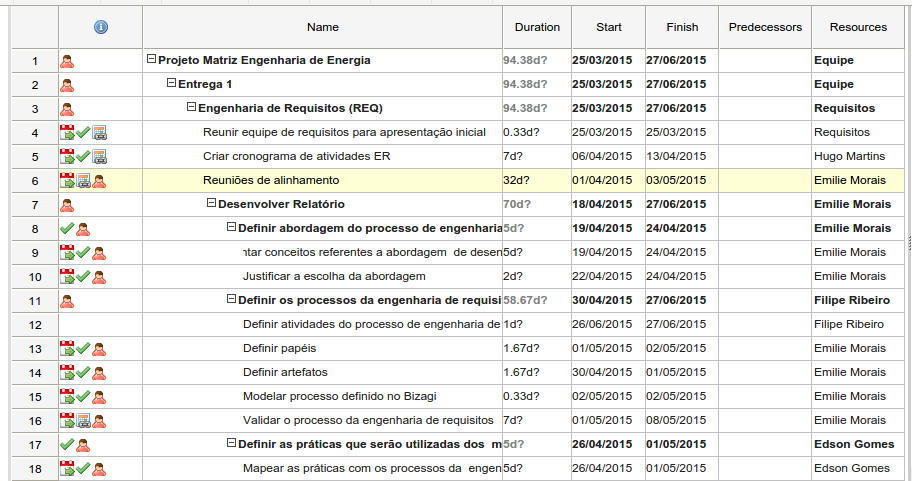
\includegraphics[scale=0.55]{figuras/cronograma1.png}
\caption{Primeira Parte do Cronograma}
\end{figure}

Neste segundo ponto do cronograma, basicamente se busca um complemento do que já foi especificado no primeiro ponto, porem, agora as atividades a serem desenvolvidas necessitam que as outras estejam concluídas.

\begin{figure}[!htb]
\centering
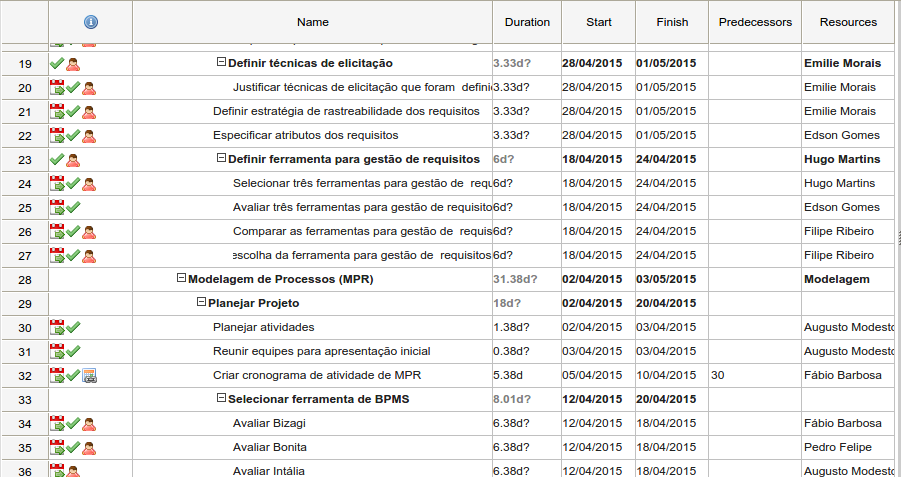
\includegraphics[scale=0.55]{figuras/cronograma2.png}
\caption{Segunda Parte do Cronograma}
\end{figure}

\begin{figure}[!htb]
\centering
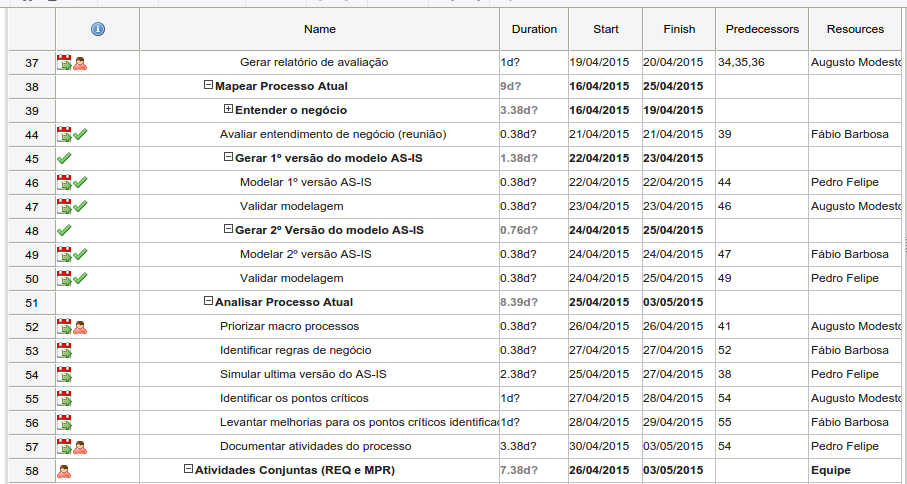
\includegraphics[scale=0.55]{figuras/cronograma3.png}
\caption{Terceira Parte do Cronograma}
\end{figure}

Com as atividades definidas e documentadas, neste ponto do projeto se busca o preparo de uma primeira apresentação como forma de visualização prévia para o grande público do que de fato sera realizado e como, além do começo das atividades referentes a segunda entrega.

\begin{figure}[!htb]
\centering
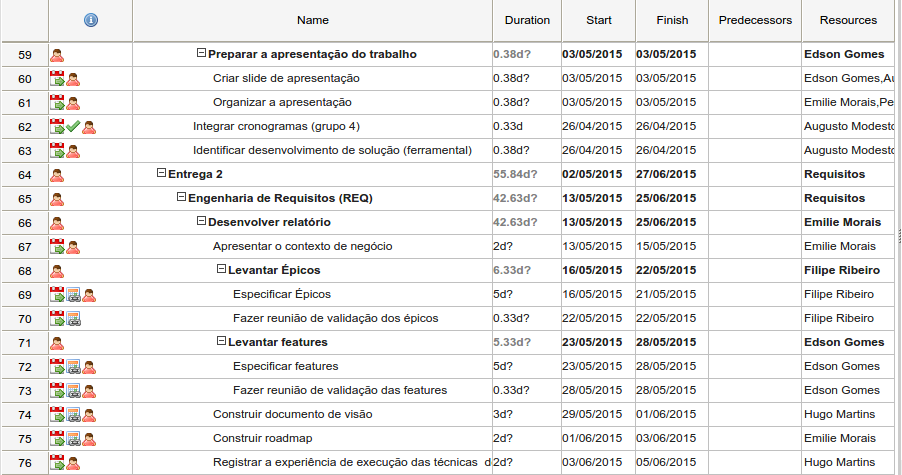
\includegraphics[scale=0.55]{figuras/cronograma4.png}
\caption{Quarta Parte do Cronograma}
\end{figure}

Dessa forma, as atividades definidas antes da entrega da primeira parte do projeto, mais precisamente na defição do projeto, serão de fato implementadas de forma prática. Haverão reuniões com a equipe de modelagem para alinhamento de trabalhos, conversas a fim de negociar novas funcionalidades etc.

\begin{figure}[!htb]
\centering
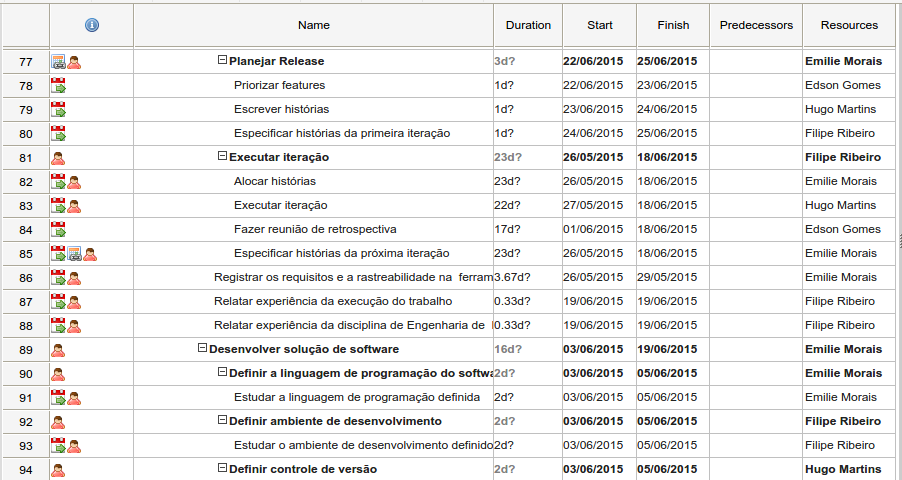
\includegraphics[scale=0.4]{figuras/cronograma5.png}
\caption{Quinta Parte do Cronograma}
\end{figure}

Por fim, a solução técnica será apresentada, e para isso necessita-se primeiro de uma detalhação de como será alcançada essa solução, via codificação ou via ferramentas BPM. Feito isso o grupo estará pronto para a apresentaçãp final.

\begin{figure}[!htb]
\centering
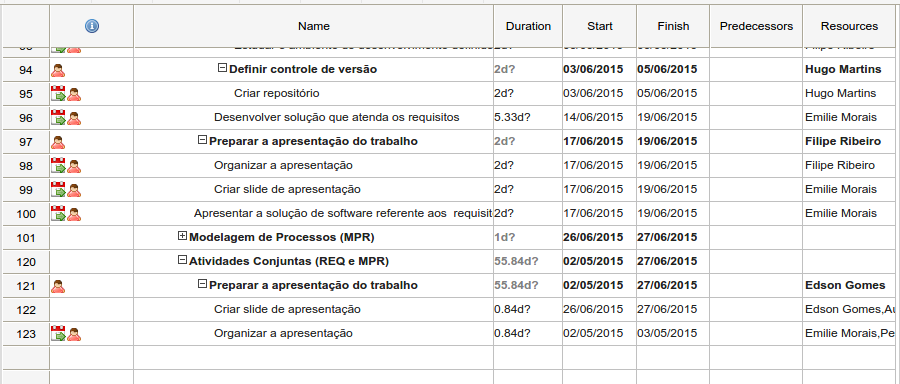
\includegraphics[scale=0.55]{figuras/cronograma6.png}
\caption{Sexta Parte do Cronograma}
\end{figure}
